\section{dram\_\-simplescalar\_\-t Class Reference}
\label{classdram__simplescalar__t}\index{dram\_\-simplescalar\_\-t@{dram\_\-simplescalar\_\-t}}
Inheritance diagram for dram\_\-simplescalar\_\-t:\nopagebreak
\begin{figure}[H]
\begin{center}
\leavevmode
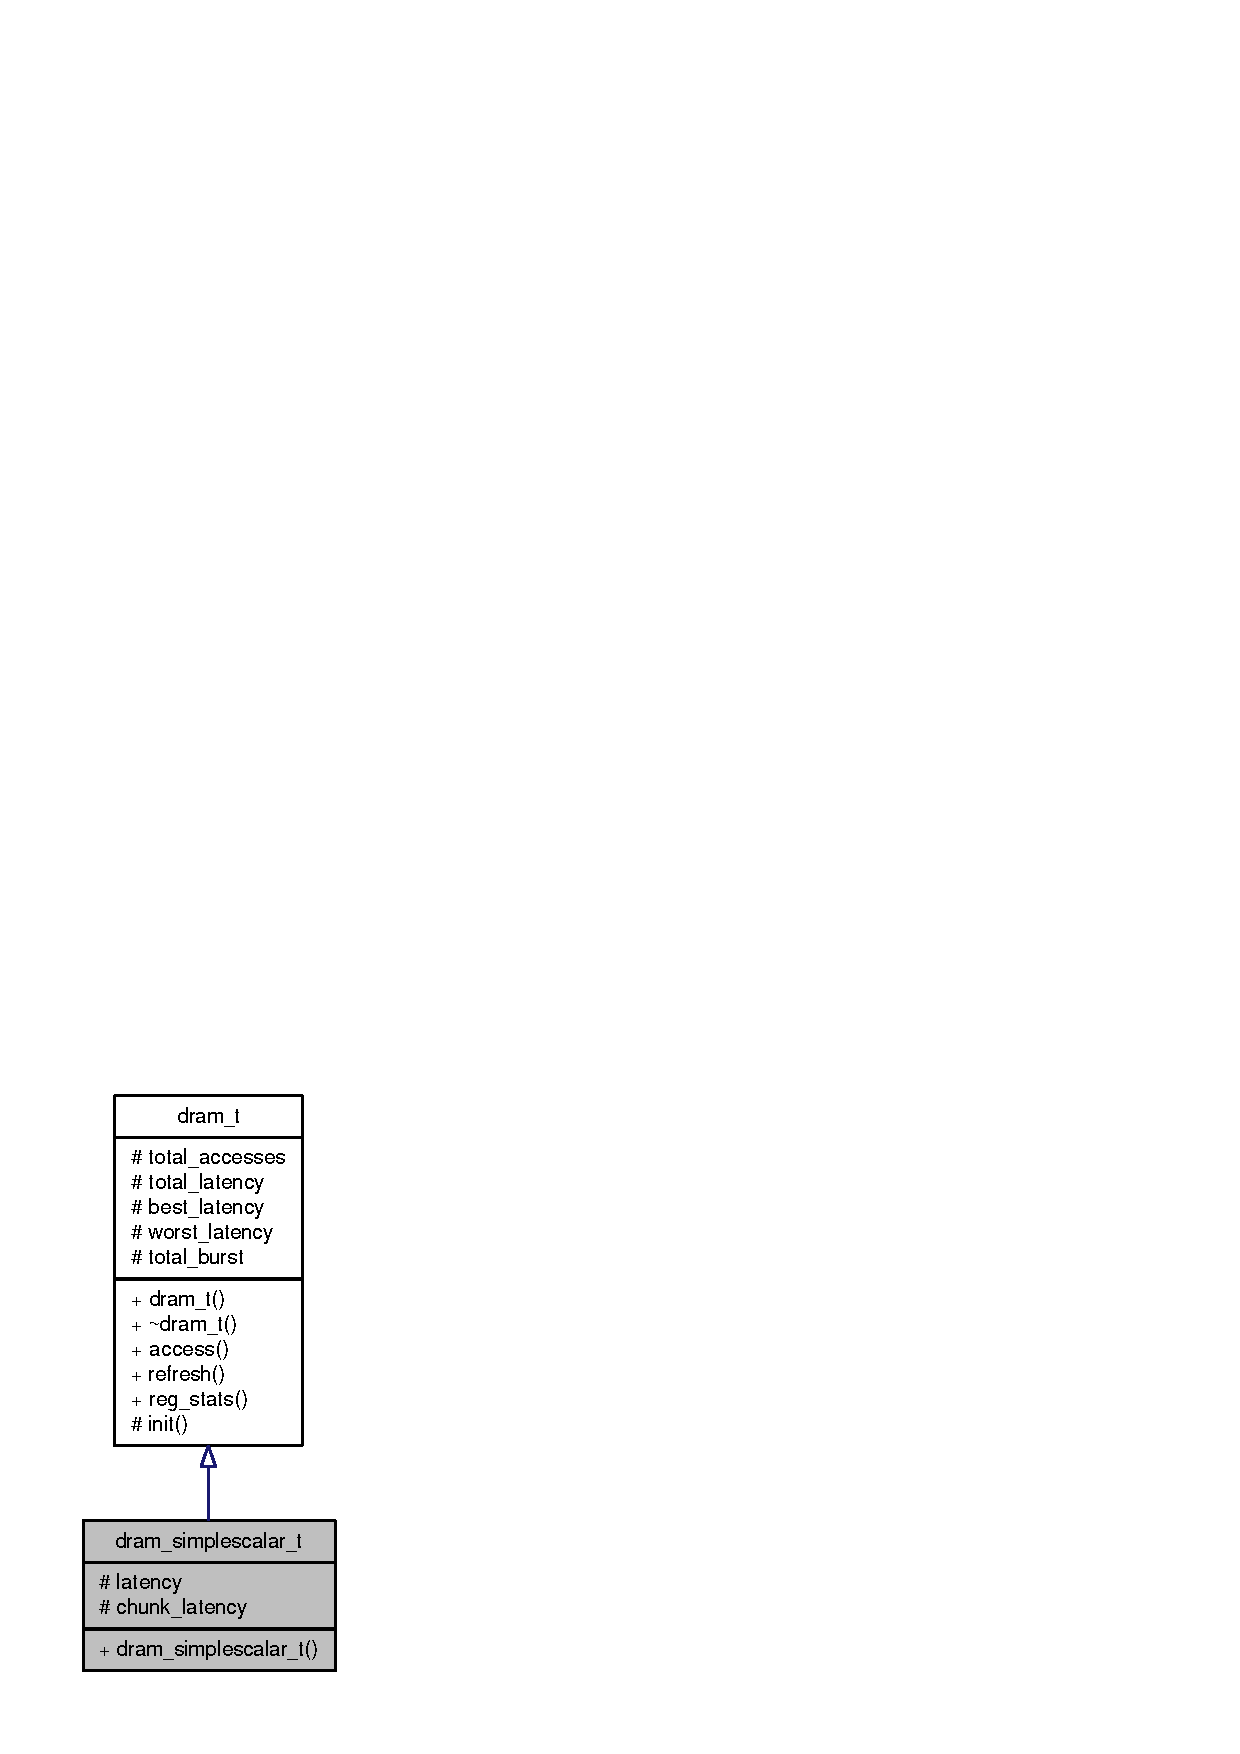
\includegraphics[width=164pt]{classdram__simplescalar__t__inherit__graph}
\end{center}
\end{figure}
Collaboration diagram for dram\_\-simplescalar\_\-t:\nopagebreak
\begin{figure}[H]
\begin{center}
\leavevmode
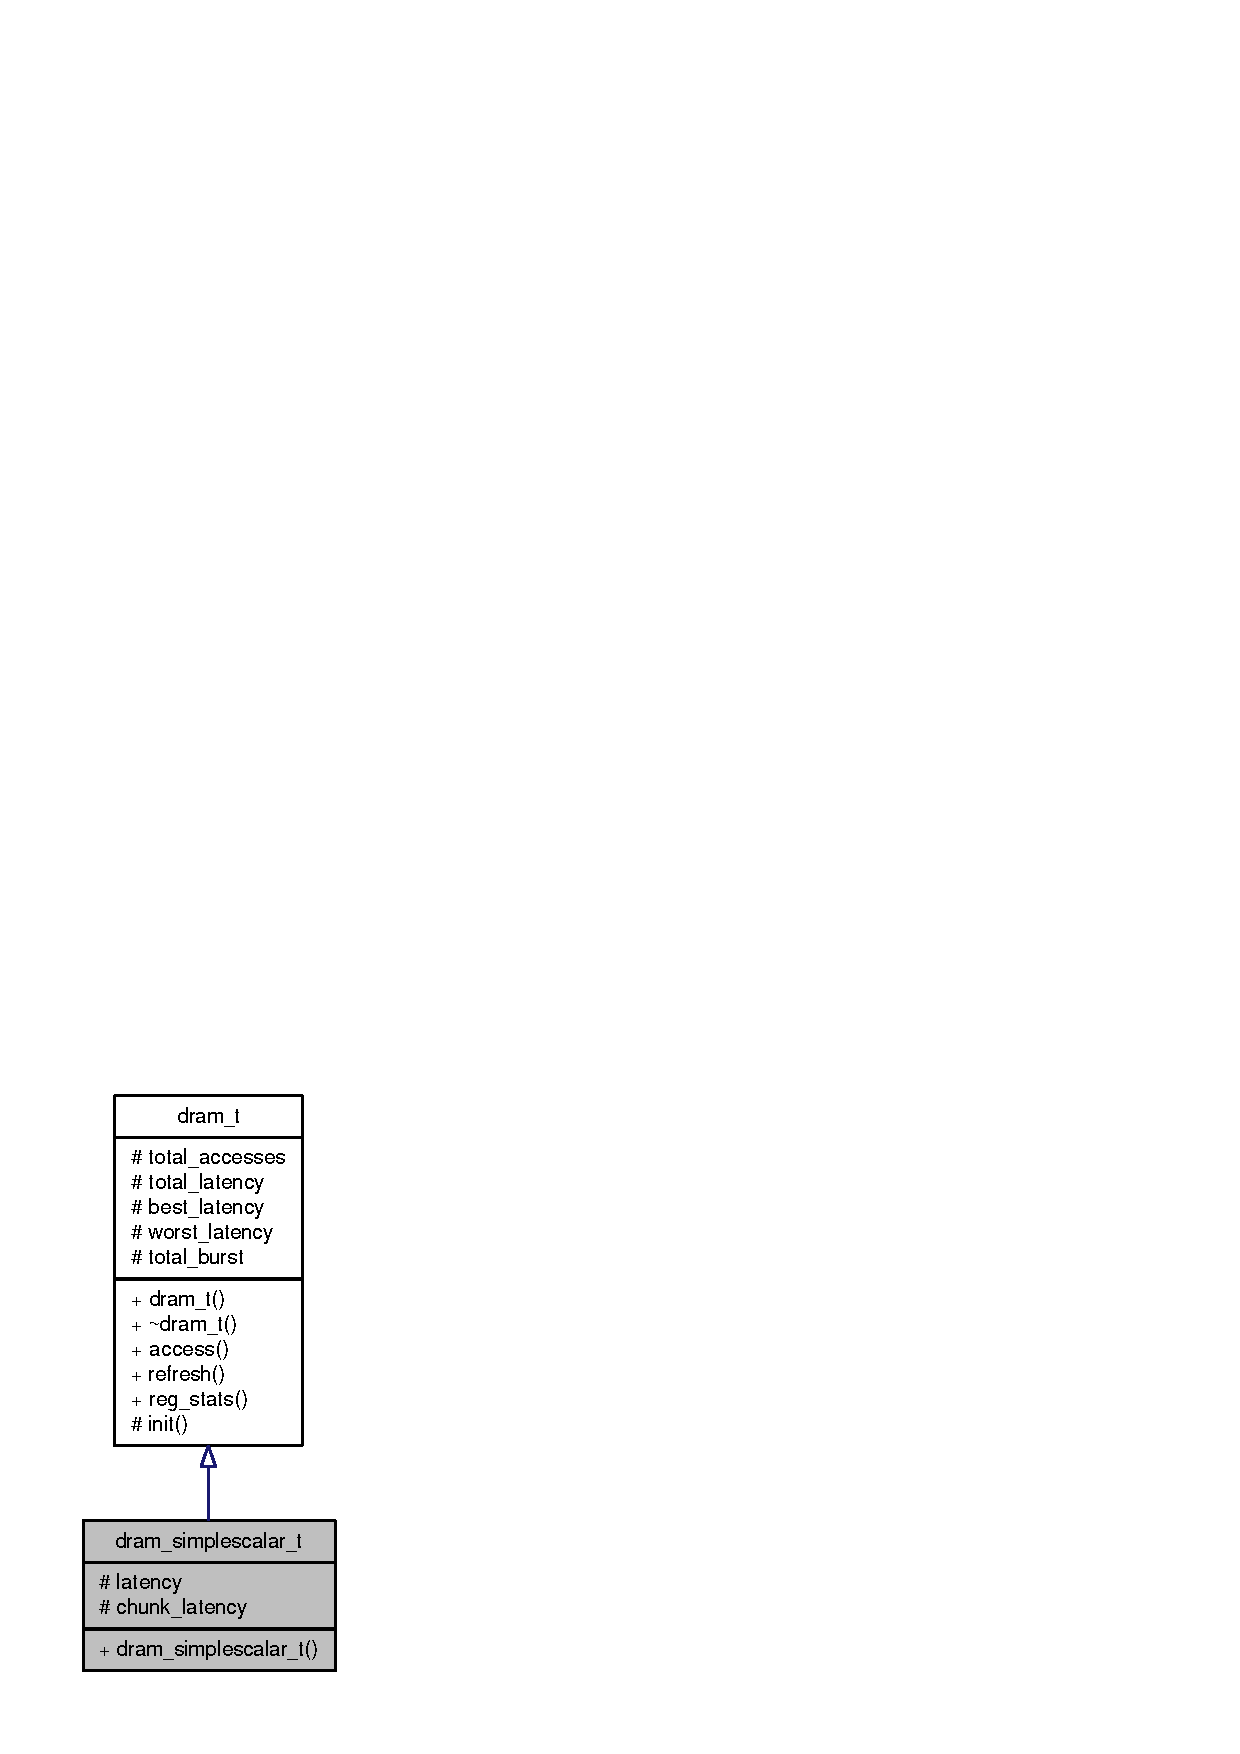
\includegraphics[width=164pt]{classdram__simplescalar__t__coll__graph}
\end{center}
\end{figure}
\subsection*{Public Member Functions}
\begin{CompactItemize}
\item 
{\bf dram\_\-simplescalar\_\-t} (int arg\_\-latency, int arg\_\-units)
\end{CompactItemize}
\subsection*{Protected Attributes}
\begin{CompactItemize}
\item 
int {\bf latency}
\item 
int {\bf chunk\_\-latency}
\end{CompactItemize}


\subsection{Detailed Description}


Definition at line 40 of file dram-simplescalar.cpp.

\subsection{Constructor \& Destructor Documentation}
\index{dram\_\-simplescalar\_\-t@{dram\_\-simplescalar\_\-t}!dram\_\-simplescalar\_\-t@{dram\_\-simplescalar\_\-t}}
\index{dram\_\-simplescalar\_\-t@{dram\_\-simplescalar\_\-t}!dram_simplescalar_t@{dram\_\-simplescalar\_\-t}}
\subsubsection[{dram\_\-simplescalar\_\-t}]{\setlength{\rightskip}{0pt plus 5cm}dram\_\-simplescalar\_\-t::dram\_\-simplescalar\_\-t (int {\em arg\_\-latency}, \/  int {\em arg\_\-units})\hspace{0.3cm}{\tt  [inline]}}\label{classdram__simplescalar__t_4c4ce8bb898ecac98ba4f9b8a05a64ed}




Definition at line 49 of file dram-simplescalar.cpp.

References dram\_\-t::best\_\-latency, chunk\_\-latency, fatal(), dram\_\-t::init(), and latency.

\subsection{Member Data Documentation}
\index{dram\_\-simplescalar\_\-t@{dram\_\-simplescalar\_\-t}!chunk\_\-latency@{chunk\_\-latency}}
\index{chunk\_\-latency@{chunk\_\-latency}!dram_simplescalar_t@{dram\_\-simplescalar\_\-t}}
\subsubsection[{chunk\_\-latency}]{\setlength{\rightskip}{0pt plus 5cm}int {\bf dram\_\-simplescalar\_\-t::chunk\_\-latency}\hspace{0.3cm}{\tt  [protected]}}\label{classdram__simplescalar__t_70c2d8e40b876b4a5a3867cb7f130147}




Definition at line 44 of file dram-simplescalar.cpp.

Referenced by dram\_\-simplescalar\_\-t().\index{dram\_\-simplescalar\_\-t@{dram\_\-simplescalar\_\-t}!latency@{latency}}
\index{latency@{latency}!dram_simplescalar_t@{dram\_\-simplescalar\_\-t}}
\subsubsection[{latency}]{\setlength{\rightskip}{0pt plus 5cm}int {\bf dram\_\-simplescalar\_\-t::latency}\hspace{0.3cm}{\tt  [protected]}}\label{classdram__simplescalar__t_0a93b5b3422346497f44ae69fc565d5b}




Definition at line 43 of file dram-simplescalar.cpp.

Referenced by dram\_\-simplescalar\_\-t().

The documentation for this class was generated from the following file:\begin{CompactItemize}
\item 
{\bf dram-simplescalar.cpp}\end{CompactItemize}
